\chapter{Minimal and Modular Jastrow Factors for the Transcorrelated Method}
\label{chap:universal}

The contents of this chapter are planned to be expanded for a future publication. Some contents may be repeated there.

\section{Introduction}

So far, the \gls{TC} methods we have discussed had one major bottleneck in common: the optimisation of the Jastrow factor. While VMC in itself does not scale unfavourably, the fact that we need so many VMC cycles in order to properly optimise for TC (see \autoref{chap:opt}) results in a significant computational cost. For large systems, this can become the prohibitive step in the workflow.

Here we explore some alternative avenues to construct Jastrow factors for use in the transcorrelated method. In particular, we consider constructing especially simple (minimal), or ``universal'' Jastrow factors that do not need any optimisation. These have already been introduced in the literature,\supercite{fournaisNonIsotropic2007,fournaisSharp2005,tewSecond2008,szenesStriking2024} and are constructed to satisfy cusp conditions. We will also construct Jastrow factors from those optimised for atomic systems. That is, we optimise the Jastrow factor for the atom, and use the same Jastrow factor for molecules (so that the molecular Jastrow is the sum of atomic Jastrows). In effect, this would allow us to compile sophisticated atomic Jastrow factors that may be stored in a database for easy retrieval when considering larger systems, without any optimisation. We also consider keeping some components of these Jastrows fixed, while optimising other elements as a ``molecular correction'' to the atomic Jastrow factor.

\section{Theory}

In this chapter, we study various choices of Jastrow factors to avoid the need for lengthy optimisation. These may be divided into two broad categories: minimal Jastrow factors and atomic Jastrow factors.

\subsection{Minimal Jastrow Factors}
\label{sec:universal-jastrow}
A minimal form for the Jastrow factor has already been presented by Fournais \emph{et al} in 2005,\supercite{fournaisSharp2005} and has occasionally made further appearances in the literature.\supercite{tewSecond2008,szenesStriking2024} The key advantage to using these is that we require no optimisation at all, while key disadvantages are that we must be careful about cut off functions, and we do not have as much flexibility so we cannot tailor the Jastrow factor to e.g. excited states.

One form of the Jastrow factor that might be called ``universal'' (that is, one that does not contain parameters that need optimisation per system)  is given by\supercite{fournaisSharp2005,fournaisNonIsotropic2007}
\begin{equation}
    \label{eq:fournais-full}
    J = -\sum_I\sum_i Z_Ir_{iI} + \frac 12\sum_{i<j}r_{ij} + \frac{2-\pi}{6\pi}\sum_I\sum_{i<j}Z_I\bm r_{iI}\cdot \bm r_{jI}\ln(r_{iI}^2+r_{jI}^2),
\end{equation}
where, as usual, upper case indices denote the nucleus, and lower case indices represent electrons. The first term resolves the electron-nucleus cusps, the second term resolves the electron-electron cusps, and finally the last term resolves electron-electron-nucleus cusps. However, these terms are unbounded, and indeed are valid only close to coalescence points. For this reason, we introduce cutoff functions on each term.

Using the form of the cutoff functions used in previous chapters, that is $t(r,L) = (1-r/L)^3\Theta(r-L)$, we find unreasonable energies even for extremely small cutoffs. For example, with this form of cutoff with the electron-nucleus and electron-electron terms, and $L=0.1$ Bohr, we get a reference energy of $-246.604$ for N$_2$ with the \avtz basis set, whereas the \gls{HEAT} result is known to be $-109.5425$.\supercite{fellerSurvey2008}

Thus, we instead use gaussian cutoffs, which are smooth but still decay rapidly for large distances. Our Jastrow factor therefore becomes % TODO : should I make a comment about smoothness? Some kind of argument other than numerics that the other cutoff does not work so well
\begin{align}
    \label{eq:fournais-full-cutoffs}
    J &= -\sum_I\sum_i Z_Ir_{iI}\e^{-r_{iI}^2/L_{en}^2} + \frac 12\sum_{i<j}r_{ij}\e^{-r_{ij}^2/L_{ee}^2} \nonumber \\
    &\quad + \frac{2-\pi}{6\pi}\sum_I\sum_{i<j}Z_I\bm r_{iI}\cdot \bm r_{jI}\ln(r_{iI}^2+r_{jI}^2)\e^{-r_{iI}^2/L_{een}^2}\e^{-r_{jI}^2/L_{een}^2},
\end{align}
where $L_{ee}, L_{en}, L_{een}$ are cutoff parameters. For this study, we take $L\mathdef L_{ee} = L_{en} = L_{een}$, and consider three variants of equation \ref{eq:fournais-full-cutoffs}:
\begin{itemize}
    \item The full analytical Jastrow factor, as in equation \ref{eq:fournais-full-cutoffs}. We shall dub this the ``Fournais-Jastrow'' factor.
    \item Neglecting the electron-electron-nucleus term and resolving the electron-nucleus cusp using the approach described in \autoref{chap:opt} (instead of via the $r_{iI}$ terms). We'll dub this the $ee+en$-Jastrow.
    \item Neglecting both the electron-electron-nucleus and electron-nucleus terms. This has already been studied in the context of TC-DMRG,\supercite{szenesStriking2024} though the choice of cutoffs may result in uncontrollably nonvariational energies. This is the simplest form, containing only $r_{ij}$ terms, and we dub it the ``$ee$-Jastrow''.
\end{itemize}

Consider again the nitrogen molecule at equilibrium. We treat the result from \gls{HEAT}\supercite{fellerSurvey2008} as the exact nonrelativistic ground state energy, and so this is as a lower bound for the lowest eigenvalue of $\htc$ for the various Jastrow factors. For each of the three choices above, there is only one parameter, $L$. For the Fournais-Jastrow factor, we find that the reference xTC-energy with a cutoff of $L=0.1$ Bohr at \avtz is $-115.122$ Hartree, which is below the HEAT result. This may be due to numerical issues from the complexity of this Jastrow factor form (none of the other ones we have explored included a dot product, for example). It may also indicate a more complex relationship between the TC energy and the cutoff $L$. As shown in \autoref{chap:opt}, the TC energy is sensitive to changes in the linear Jastrow factor parameters. As this term appears nonlinearly, determining $L$ may be more challenging. However, for vanishingly small $L$, the TC and non-TC energies should be roughly equal. Even at $L=0.1$ Bohr this is not the case, implying that for the Fournais-Jastrow factor, the TC energy is particularly sensitive to the choice of cutoff. Therefore, for simplicity, we exclude the Fournais-Jastrow factor from this study and consider only the $ee$- and $ee+en$-Jastrow factors.

The energy of N$_2$ and N with the \avtz basis set for the $ee$- and $ee+en$-Jastrow factors are shown in figure \ref{fig:fournais-cutoff-n2}. Shown are three non-TC energies: the canonical (RHF) reference energy, the canonical FCIQMC energy, and the HEAT (effectively \gls{CBS}) energy. Plotted as a function of $L$ are three TC energies, the xTC (RHF) reference energy, the xTC-MP2 energy, and the xTC-FCIQMC energy. For small $L$, we expect the non-TC- and xTC- reference and FCIQMC energies to coincide, which they approximately do. In contrast, for large $L$ we expect the energies to become unstable, as we start to include spurious long-range correlation. However, it is worth noting that according to these plots, ``long-range'' is already at $\approx 0.4$ Bohr, as the energies are all below the HEAT result. In every case, $L=0.3$ Bohr is shown to result in energies above that of HEAT but below that of non-TC. We therefore use $L=0.3$ Bohr as our ``universal'' cutoff for these Jastrow factors.

\begin{figure}[h!]
    \centering
    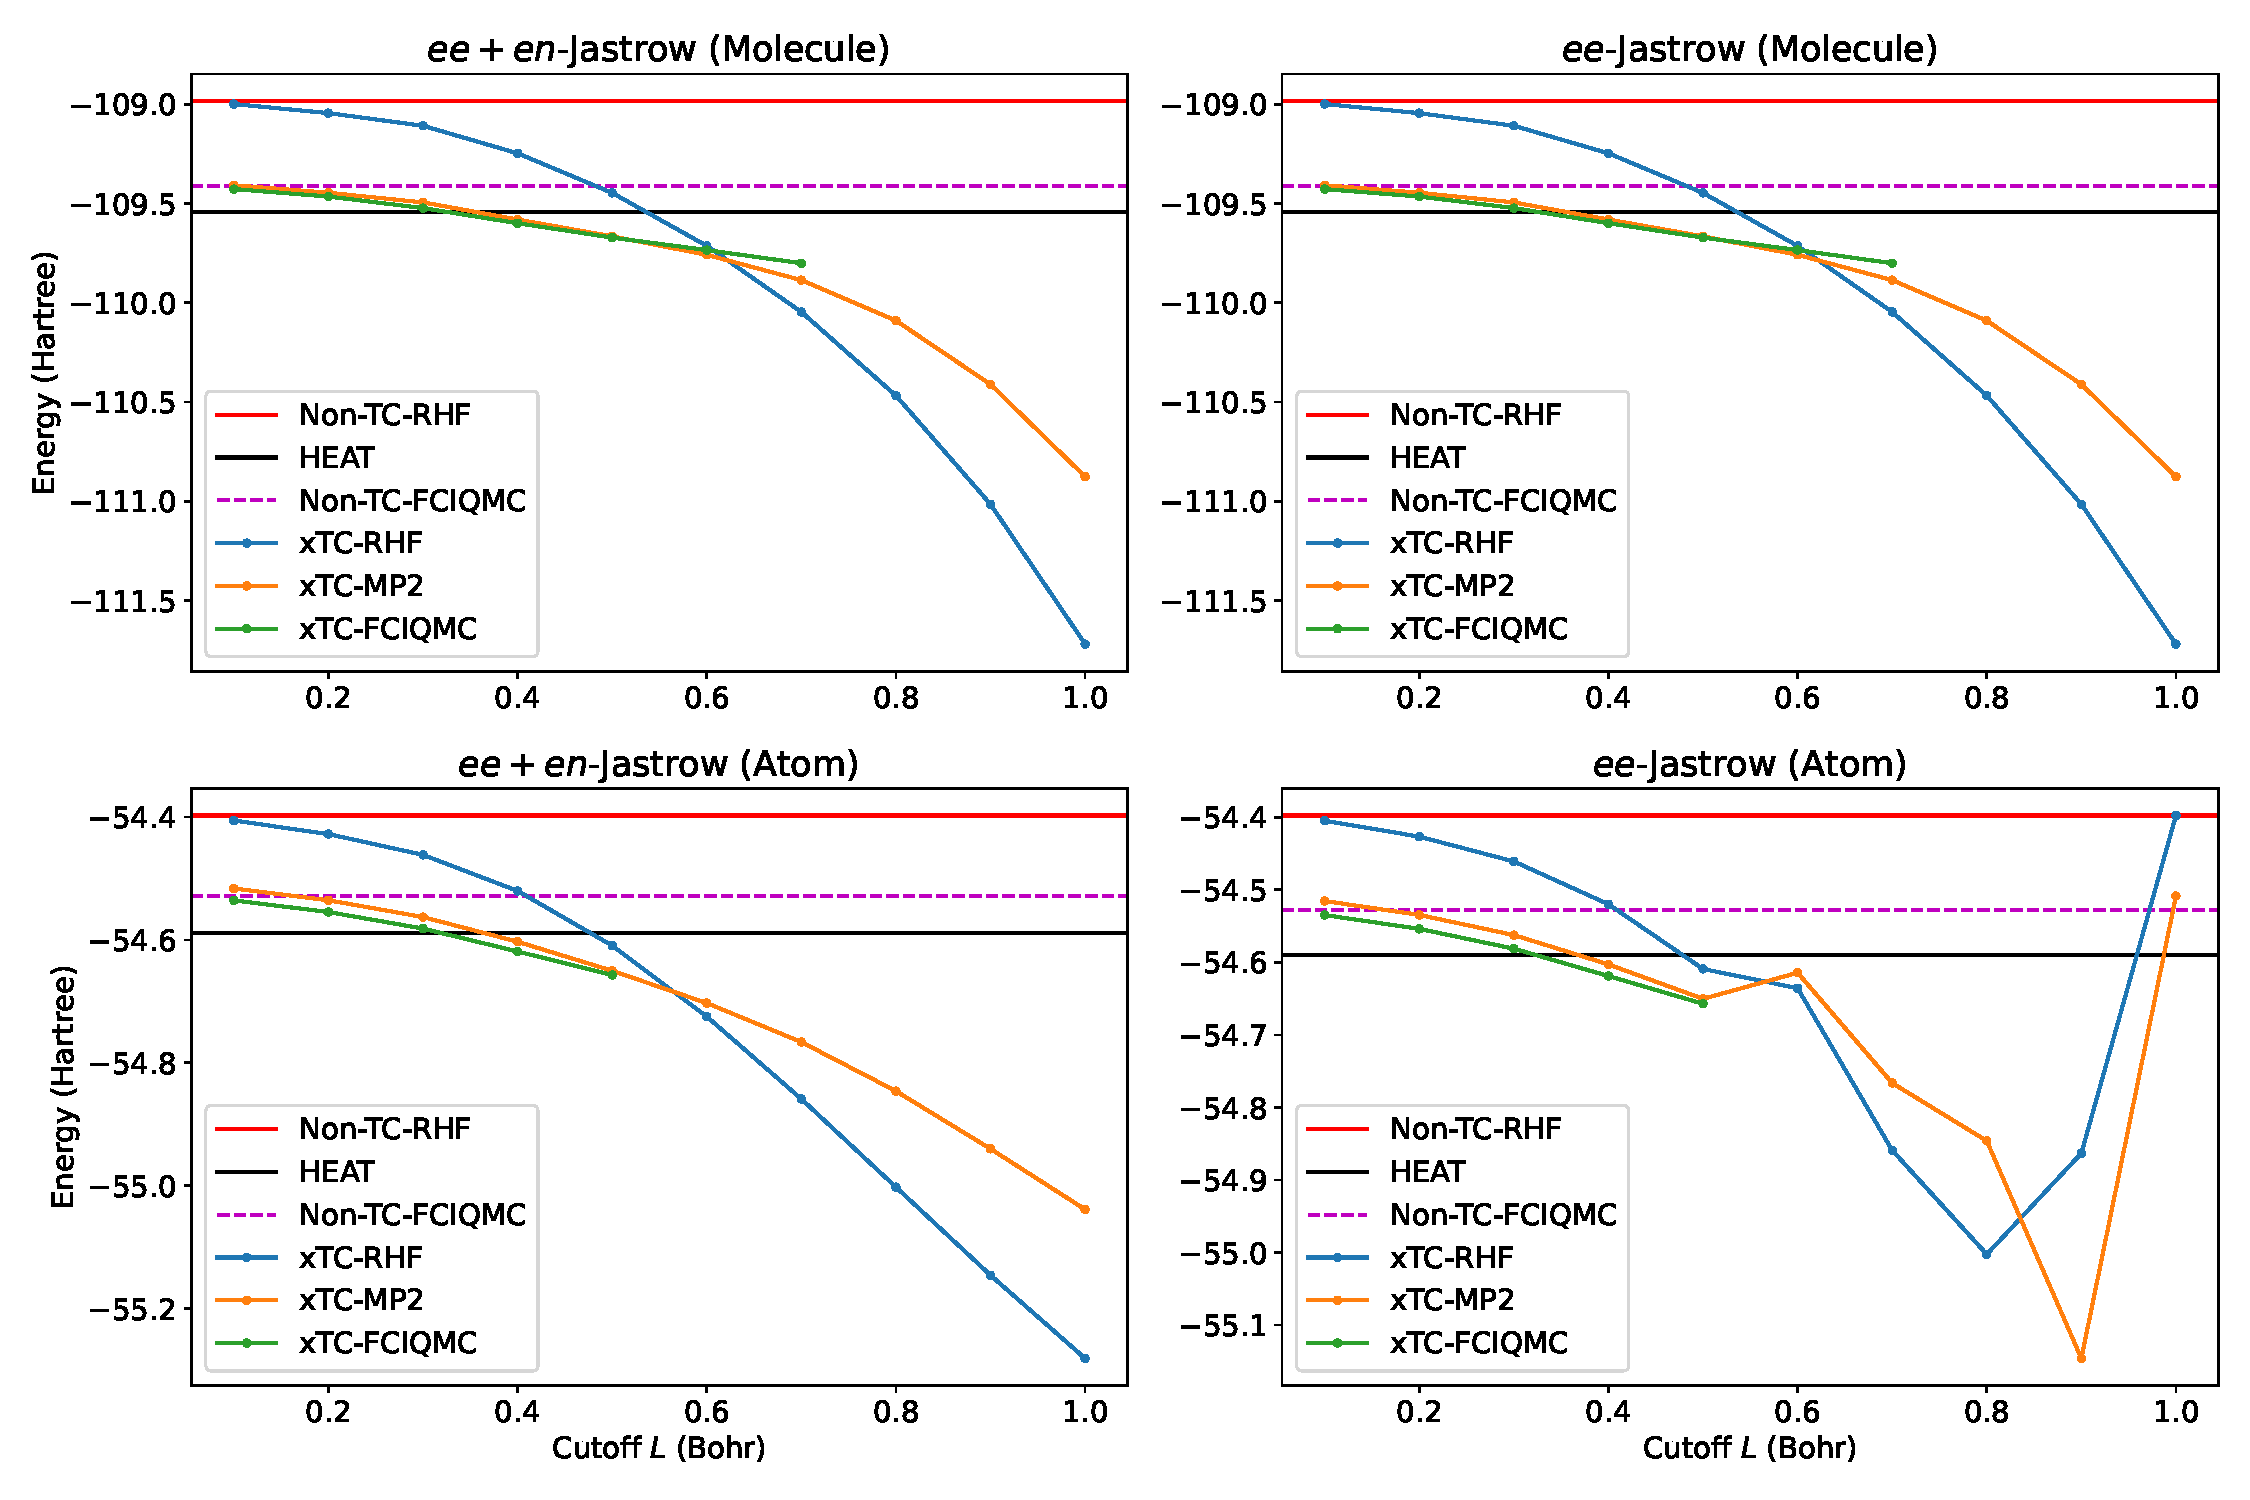
\includegraphics[width=\textwidth]{figures/universal/cutoffs_combined}
    \caption{Energy estimates for the nitrogen molecule (top panel) and atom (bottom panel) as a function of a cutoff parameter $L$ for the $ee+en$- (left panel) and $ee$-Jastrow (right panel) factors. The non-TC reference (RHF) energies are represented by a horizontal red line, the HEAT result by a horizontal black line, and the non-TC-FCIQMC by a dashed line.
    Since HEAT is a \gls{CBS}-extrapolated method, and variational theories are typically preferred, we aim to keep our TC energies above this value. However, we also expect TC to improve upon the canonical FCIQMC energy.
    We therefore take the value of $L$ that leads to energies above the HEAT result, which is $L=0.3$ for all four plots. Large- and small-$L$ limits behave as expected, with the former giving undesirable results and the latter approximating the non-TC results in that basis set. All calculations were performed with the \avtz basis set. Missing xTC-FCIQMC points are due to numerical instability caused by a positive correlation energy. In practice, these may be resolved by setting a positive shift, but these results are anyway undesirable. Noise caused by the large cutoff in the $ee$-Jastrow factor for the atom likely indicates unfavourable changes to the one-electron density encoded in the HF orbitals. Adding an electron-nucleus term has been known to give a stabilising effect counteracting this,\supercite{needsVariational2020,boysCalculation1969}, which is consistent with the fact that the $ee+en$-Jastrow factor does not exhibit this noise.}
    \label{fig:fournais-cutoff-n2}
\end{figure}

Since TC amounts to a similarity transformation, and any similarity transformation exactly preserves the eigenspectrum in the CBS limit, we know that this undesirable behaviour must be a basis set effect. Moreover, since the effects of these Jastrow factors are extremely localised near the nuclei, we might expect core-valence basis functions to aid in the TC energies. Figure \ref{fig:basis-vs-cutoff} shows the effect of adding core functions to the basis set for the $ee+en$-Jastrow factor. We see that the core functions increase the (positive) correlation energies to bring it closer to the CBS limit, as does increasing the size (cardinal number) of the basis set. However, even cc-pCVQZ is not enough to bring the xTC-MP2 energy above the HEAT result for cutoff values above 0.4 Bohr. This suggests a very strong basis set effect, and merits further studies.

\begin{figure}[h!]
    \centering
    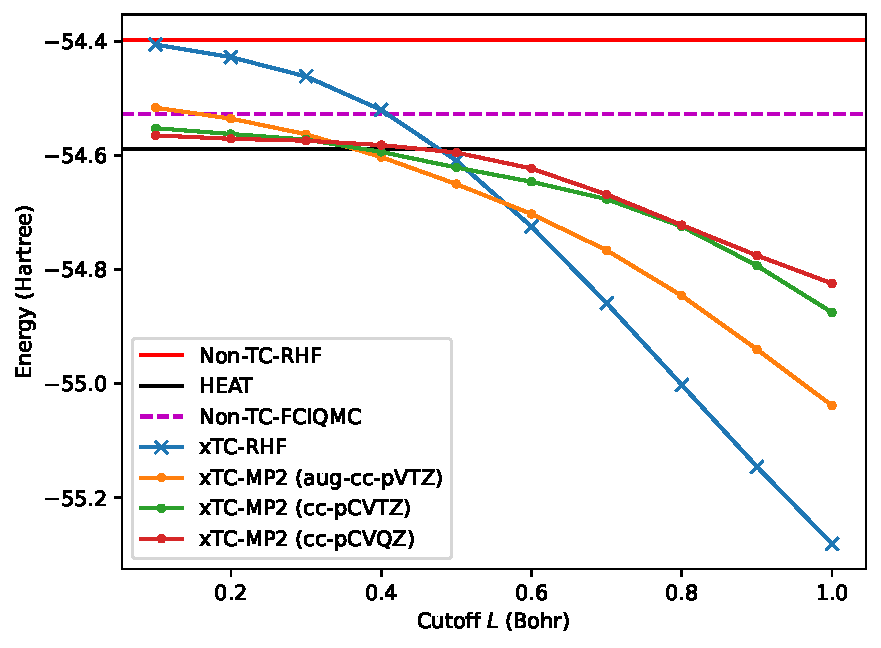
\includegraphics[width=0.8\textwidth]{figures/universal/cutoffs_basis.pdf}
    \caption{MP2 energies as a function of the cutoff $L$ for the $ee+en$-Jastrow factor. The xTC-RHF values are roughly the same for each basis set shown. Adding core functions significantly improves the curve to be closer to the HEAT result, resulting in larger (positive) correlation energies. Increasing the cardinal number of the basis set also improves the curve, but the effect is less pronounced. Nevertheless, these results indicate a strong basis set effect in the cutoff, particularly for core functions.
    Adding diffuse functions have negligible effects on the curve (e.g. xTC-MP2 curves for aug-cc-pCVTZ, not shown here, and cc-pCVTZ roughly coincide).}
    \label{fig:basis-vs-cutoff}
\end{figure}

\subsection{Atomic Jastrow Factors}

Another approach we consider in reducing the need for optimisation is to optimise Jastrow factors for atomic systems and then reuse them in the molecular context. This can be considered analogous to mixing atomic orbitals orbitals in order to calculate molecular orbitals. The key advantage here is flexibility while the key disadvantages include the need to optimise for the atoms, and the need to make a choice for the form of the Jastrow factor. In principle, we could produce a database of sophisticated atomic Jastrow factors that can then be queried to construct Jastrow factors for molecules or periodic systems. We use the Jastrow forms considered earlier in this dissertation, \begin{equation}
    \label{eq:jastrow-3}
    J = \sum_{i<j}^Nv(r_{ij}) + \sum_i^N\sum_I^{N_A}\chi(r_{iI}) + \sum_{i<j}^N\sum_I^{N_A}f(r_{ij}, r_{iI}, r_{jI}),
\end{equation}
with
\begin{equation}
    \label{eq:dtn-jastrow-ee-3}
    v(r_{ij})    = t(r_{ij},L_v)
                    \sum_{k} a_k r_{ij}^k ,
\end{equation}
\begin{equation}
    \label{eq:dtn-jastrow-en-3}
    \chi(r_{iI}) = t(r_{iI},L_\chi)
    \sum_{k} b_k r_{iI}^k ,
\end{equation}
\begin{equation}
    \label{eq:dtn-jastrow-een-3}
    f(r_{ij}, r_{i}, r_{j}) = t(r_{iI},L_f) t(r_{jI},L_f)
    \sum_{k,l,m} c_{klm}
    r_{ij}^k r_{iI}^l r_{jI}^m ,
\end{equation}
and the same cutoff functions $t(r,L) = (1-r/L)^3
\Theta(r-L)$. However, we do not want to include long-range (with respect to the nucleus) correlation in the atomic Jastrow factors, since this may bias the molecular calculations. We therefore use $L_f=L_\chi=1.0$ Bohr and $L_{v}=4.5$ Bohr. We consider the following variants:
\begin{itemize}
    \item The Jastrow factor is kept constant for the molecule, i.e. we simply use the atomic Jastrow factors as they are. We refer to these as simply ``atomic'' Jastrow factors.
    \item We optimise the atomic Jastrow factor using all terms. Then, when calculating molecules, we fix all terms involving nuclei and re-optimise the electron-electron terms. We refer to these as ``atomic$+ee$'' Jastrow factors.
\end{itemize}

We find these to yield results above HEAT and therefore do not concern ourselves with a cutoff analysis as in the case of the minimal Jastrow factors.

\section{Results}

\subsection{Computational Details}

We revisit the nitrogen binding curve from \autoref{chap:binding} as a stress test for our Jastrow factors, as well as the atomisation of the molecules N$_2$, C$_2$, O$_2$, and CN from \autoref{chap:opt}. As before, we compare the results of the different choices of Jastrow factors against experiment\supercite{leroyAccurate2006} and the atomisation energies to HEAT.\supercite{fellerSurvey2008} The binding curve is calculated with the \avtz basis set, while the atomisation energies are calculated with the \avxz{$X$} basis sets for $X=\text{D},\text{T},\text{Q}$.

For the multideterminantal optimisation, we use a small FCIQMC calculation as it was found to perform particularly well in \autoref{chap:binding}. Non-TC HF and CASCI calculations were performed using \pyscf,\supercite{sunPySCF2018} VMC optimisation was performed using \casino,\supercite{needsVariational2020} FCIQMC calculations using \neci,\supercite{gutherNECI2020} and MRCI-F12 calculations for comparison using \molpro.\supercite{wernerMOLPRO,wernerMolpro2012,wernerMolproQuantumChemistry2020}


\subsection{Atomisation Energies}
\label{sec:universal-atomisation}

For the atomisation energies, we focus on the $ee+en$ and atomic$+ee$ Jastrow factors, as these are the most ``complete'' of each category of Jastrow factors presented here. The absolute xTC-FCIQMC energy estimates using the various methods for the systems considered in this chapter are presented in table \ref{tbl:universal-absE}. Also presented there are the non-TC FCIQMC and TC-FCIQMC (that is, with no additional approximations such as xTC), as presented in \autoref{chap:opt}.

\begin{table}[htbp]
    \centering
    \begin{tabular}{c|c|ccc||c}
    System & Method & \vdz & \vtz & \vqz & \gls{CBS}\supercite{fellerSurvey2008,bytautasCorrelation2005} \\
    \hline
    \multirow{4}{*}{N$_2$} & Non-TC & -109.2809 & -109.4014 & -109.4653 & \multirow{4}{*}{-109.5425} \\
      & Full TC & -109.4727 & -109.5312 & -109.5428 &  \\
      & $ee+en$ & -109.4125 & -109.5141 & \red{-109.5580} &  \\
      & Atomic+$ee$ & -109.4364 & -109.5168 & -109.5410 &  \\
    \hline
    \multirow{4}{*}{C$_2$} & Non-TC & -75.7320 & -75.8094 & -75.8578 & \multirow{2}{*}{-75.9240} \\
    & Full TC & -75.8844 & -75.9197 & \red{-75.9272} &  \\
    & $ee+en$ & -75.8153 & -75.8823 & -75.9248 & \multirow{2}{*}{-75.9265}  \\
    & Atomic+$ee$ & -75.8567 & -75.9082 & -75.9248 &  \\
    \hline
    \multirow{4}{*}{O$_2$} & Non-TC & -149.9915 & -150.1554 & -150.2362 & \multirow{4}{*}{-150.3273} \\
    & Full TC & -150.2216 & -150.3078 & -150.3244 &  \\
    & $ee+en$ & -150.1972 & -150.3243 & \red{-150.3662} &  \\
    & Atomic+$ee$ & -150.1763 & -150.2908 & -150.3221 &  \\
    \hline
    \multirow{4}{*}{CN} & Non-TC & -92.4970 & -92.5954 & -92.6517 & \multirow{4}{*}{-92.7232} \\
    & Full TC & -92.6671 & -92.7152 & -92.7247 &  \\
    & $ee+en$ & -92.6039 & -92.6872 & \red{-92.7281} & \\
    & Atomic+$ee$ & -92.6331 & -92.6992 & -92.7205 & \\
    \hline\hline
    \multirow{4}{*}{N} & Non-TC & -54.4801 & -54.5252 & -54.5535 & \multirow{4}{*}{-54.5893} \\
    & Full TC &  -54.5622 & -54.5842 & -54.5896  \\
    & $ee+en$ & -54.5425 & -54.5792 & \red{-54.5986} & \\
    & Atomic+$ee$ & -54.5477 & -54.5786 & -54.5890 & \\
    \hline
    \multirow{4}{*}{C} & Non-TC & -37.7619 & -37.7900 & -37.8126 & \multirow{4}{*}{-37.8450} \\
    & Full TC & -37.8293 & -37.8427 & -37.8459 & \\
    & $ee+en$ & -37.8020 & -37.8256 & -37.8437 &  \\
    & Atomic+$ee$ & -37.8193 & -37.8374 & -37.8451 &  \\
    \hline
    \multirow{4}{*}{O} & Non-TC & -74.9117 & -74.9853 & -75.0236 & \multirow{4}{*}{-75.0674} \\
    & Full TC & -75.0226 & -75.0572 & -75.0665 &  \\
    & $ee+en$ & -75.0123 & -75.0686 & \red{-75.0882} &  \\
    & Atomic+$ee$ & -74.9986 & -75.0514 & -75.0657 &  \\
    \end{tabular}
    \caption{
    Absolute energies for N$_2$, C$_2$, O$_2$, CN, N, O, and C using conventional non-TC-FCIQMC, the full TC workflow with larger cutoffs (see \autoref{chap:opt}), the minimal $ee+en$ Jastrow factor with $L=0.3$ Bohr, and the atomic$+ee$ Jastrow factor, where the Jastrow factors for the atoms are reused for the molecule, and the $ee$ term is reoptimised with the RHF molecular wave function ansatz. Values are reported in Hartree for the \vdz, \vtz and \vqz basis sets and compared against high-accuracy benchmarks.\supercite{fellerSurvey2008,bytautasCorrelation2005} We find that all TC methods converge rapidly to the CBS limit, but the $ee+en$ Jastrow factor has a tendency to ``overshoot'' the limit at \vqz, suggesting a nonlinear convergence. Values in red are below the CBS limit. This only occurs at \vqz with the minimal Jastrow factor; the atomic Jastrow factor is more stable, and is the only TC method presented to consistently be above the energy at the CBS limit.
    }
    \label{tbl:universal-absE}
\end{table}

From this table, it is clear that all the TC methods have much more rapid convergence toward the \gls{CBS} limit. The ``full TC'' method, as presented in \autoref{chap:opt} which uses the form of equation \ref{eq:jastrow-3} with larger cutoff values (4.5, 4 and 4 Bohr for the electron-electron, electron-nucleus and electron-electron-nucleus terms, respectively) converges to the CBS limit most rapidly, as expected. The atomic$+ee$ total energies also converge to the CBS limit much more rapidly than conventional FCIQMC, and is remarkably close at \vqz. While the absolute energies for the molecules still differ from the CBS limit by up to about 5 mHa in the \vqz basis, all atom calculations are within 1 mHa of the CBS limit.

The (minimal) $ee+en$-Jastrow factor also exhibits rapid basis set convergence, but unlike the other methods also results in energies below the CBS limit with the \vqz basis set. These discrepencies can be quite large, almost 40 mHa in the case of CN. This might suggest that our ``universal'' cutoff proposed in figure \ref{fig:fournais-cutoff-n2} really is not so ``universal'' after all. The $L$ chosen was not properly optimised, and was determined using only one system, so it is not wholly surprising that we might get questionable TC final energies using it.

However, in practice we are typically much more interested in relative energies. The atomisation energies for these molecules, obtained from the values in table \ref{tbl:universal-absE} are shown in table \ref{tbl:universal-atomisation} and plotted in figure \ref{fig:universal-atomisation}.
We find that despite the nonvariational energies found in table \ref{tbl:universal-absE}, error cancellation when using the $ee+en$ terms are enough to give sensible atomisation energy estimates. However, they are consistently outperformed by the atomic$+ee$ Jastrow factor, which is also a relatively inexpensive calculation due to the lack of additional terms needed to be optimised. This data suggests to use Jastrow factors based on atomic systems for systems that are not amenable to VMC calculations for all parameters.

As with the total energies, the TC atomisation energies converge much faster with respect to basis-set size in comparison to the non-TC calculations. While not quite on par with the other TC methods, it appears to converge faster with respect to basis set size than the non-TC energies. Nevertheless, the uncontrolled nonvariational error arising from a fixed $L$ value suggests caution when considering the use of such minimal Jastrow factors. In contrast, the atomic$+ee$ is much more robust.


\begin{table}[htbp]
    \centering
    \begin{tabular}{c|c|ccc||c}
    Molecule & Method & \vdz & \vtz & \vqz & \gls{CBS}\supercite{fellerSurvey2008} \\
    \hline
    \multirow{4}{*}{N$_2$} & Non-TC &320.7 & 351.0 & 358.3 &
    \multirow{4}{*}{363.9} \\
      & Full TC & 348.3 & 362.8 & \textbf{363.6} &  \\
      & $ee+en$ & 327.6 & 355.6 & 360.9 &  \\
      & Atomic+$ee$ & 341.0 & 359.7 & \textbf{363.0} &  \\
    \hline
    \multirow{4}{*}{C$_2$} & Non-TC & 208.2 & 229.4 & \textbf{232.6} &
    \multirow{2}{*}{234.0} \\
    & Full TC & 225.8 & 234.3 & \textbf{235.4} &   \\
    & $ee+en$ & 211.3 & 231.1 & \textbf{233.9} & \multirow{2}{*}{236.5}   \\
    & Atomic+$ee$ & 218.1 & 233.4 & \textbf{234.5} & \\
    \hline
    \multirow{4}{*}{O$_2$} & Non-TC & 168.1 & 184.8 & 189.0 &\multirow{4}{*}{192.5} \\
    & Full TC & 176.4 & 193.4 & \textbf{191.4} &   \\
    & $ee+en$ & 172.6 & 187.2 & 189.7 &    \\
    & Atomic+$ee$ & 179.0 & 188.1 & 190.7 &    \\
    \hline
    \multirow{4}{*}{CN} & Non-TC & 255.0 & 280.2 & 285.6 & \multirow{4}{*}{288.9} \\
    & Full TC & 275.6 & 288.3 & \textbf{289.2} &  \\
    & $ee+en$ & 259.5 & 282.3 & 285.8 &  \\
    & Atomic+$ee$ & 266.1 & 283.2 & 286.4 &  \\
    \end{tabular}
    \caption{Atomisation energies for N$_2$, C$_2$, O$_2$ and CN. Results are shown for the $ee+en$ and atomic$+ee$ Jastrow factors, and compared to non-TC and full TC for the \vdz, \vtz and \vqz basis sets, as well as to the CBS limit. Bold face indicates being within chemical accuracy of one of the benchmark CBS values.
    % We find that despite the nonvariational energies found in table \ref{tbl:universal-absE}, error cancellation when using the $ee+en$ terms are enough to give sensible atomisation energy estimates. However, they are consistently outperformed by the atomic$+ee$ Jastrow factor, which is also a relatively inexpensive calculation due to the lack of additional terms needed to be optimised. This data suggests to use Jastrow factors based on atomic systems for systems that are not amenable to VMC calculations for all parameters.
    }
    \label{tbl:universal-atomisation}
\end{table}

Unlike with full TC, the atomic and minimal Jastrow factors presented do not consistently reach chemical accuracy (defined as within 1.6 mHa of the value at the CBS limit) for the atomisation of any molecules. However, they are still considerably closer than non-TC. Moreover, the atomic Jastrow factor consistently outperforms the minimal form. Since, as discussed, this form also gives absolute energies above the CBS limit, converging from above, this is strong evidence that the atomic$+ee$ Jastrow factor form is the preferred method for systems that are too large for optimising all parameters simultaneously as done in previous chapters. While we have reduced accuracy, the trade off of not needing to calculate all parameters may be worthwhile for future applications of the TC method. In the full TC calculations, the Jastrow factors had 44 optimisable parameters; in the atomic$+ee$ case, there are only 8 optimisable parameters.



\begin{figure}[htbp]
    \centering
    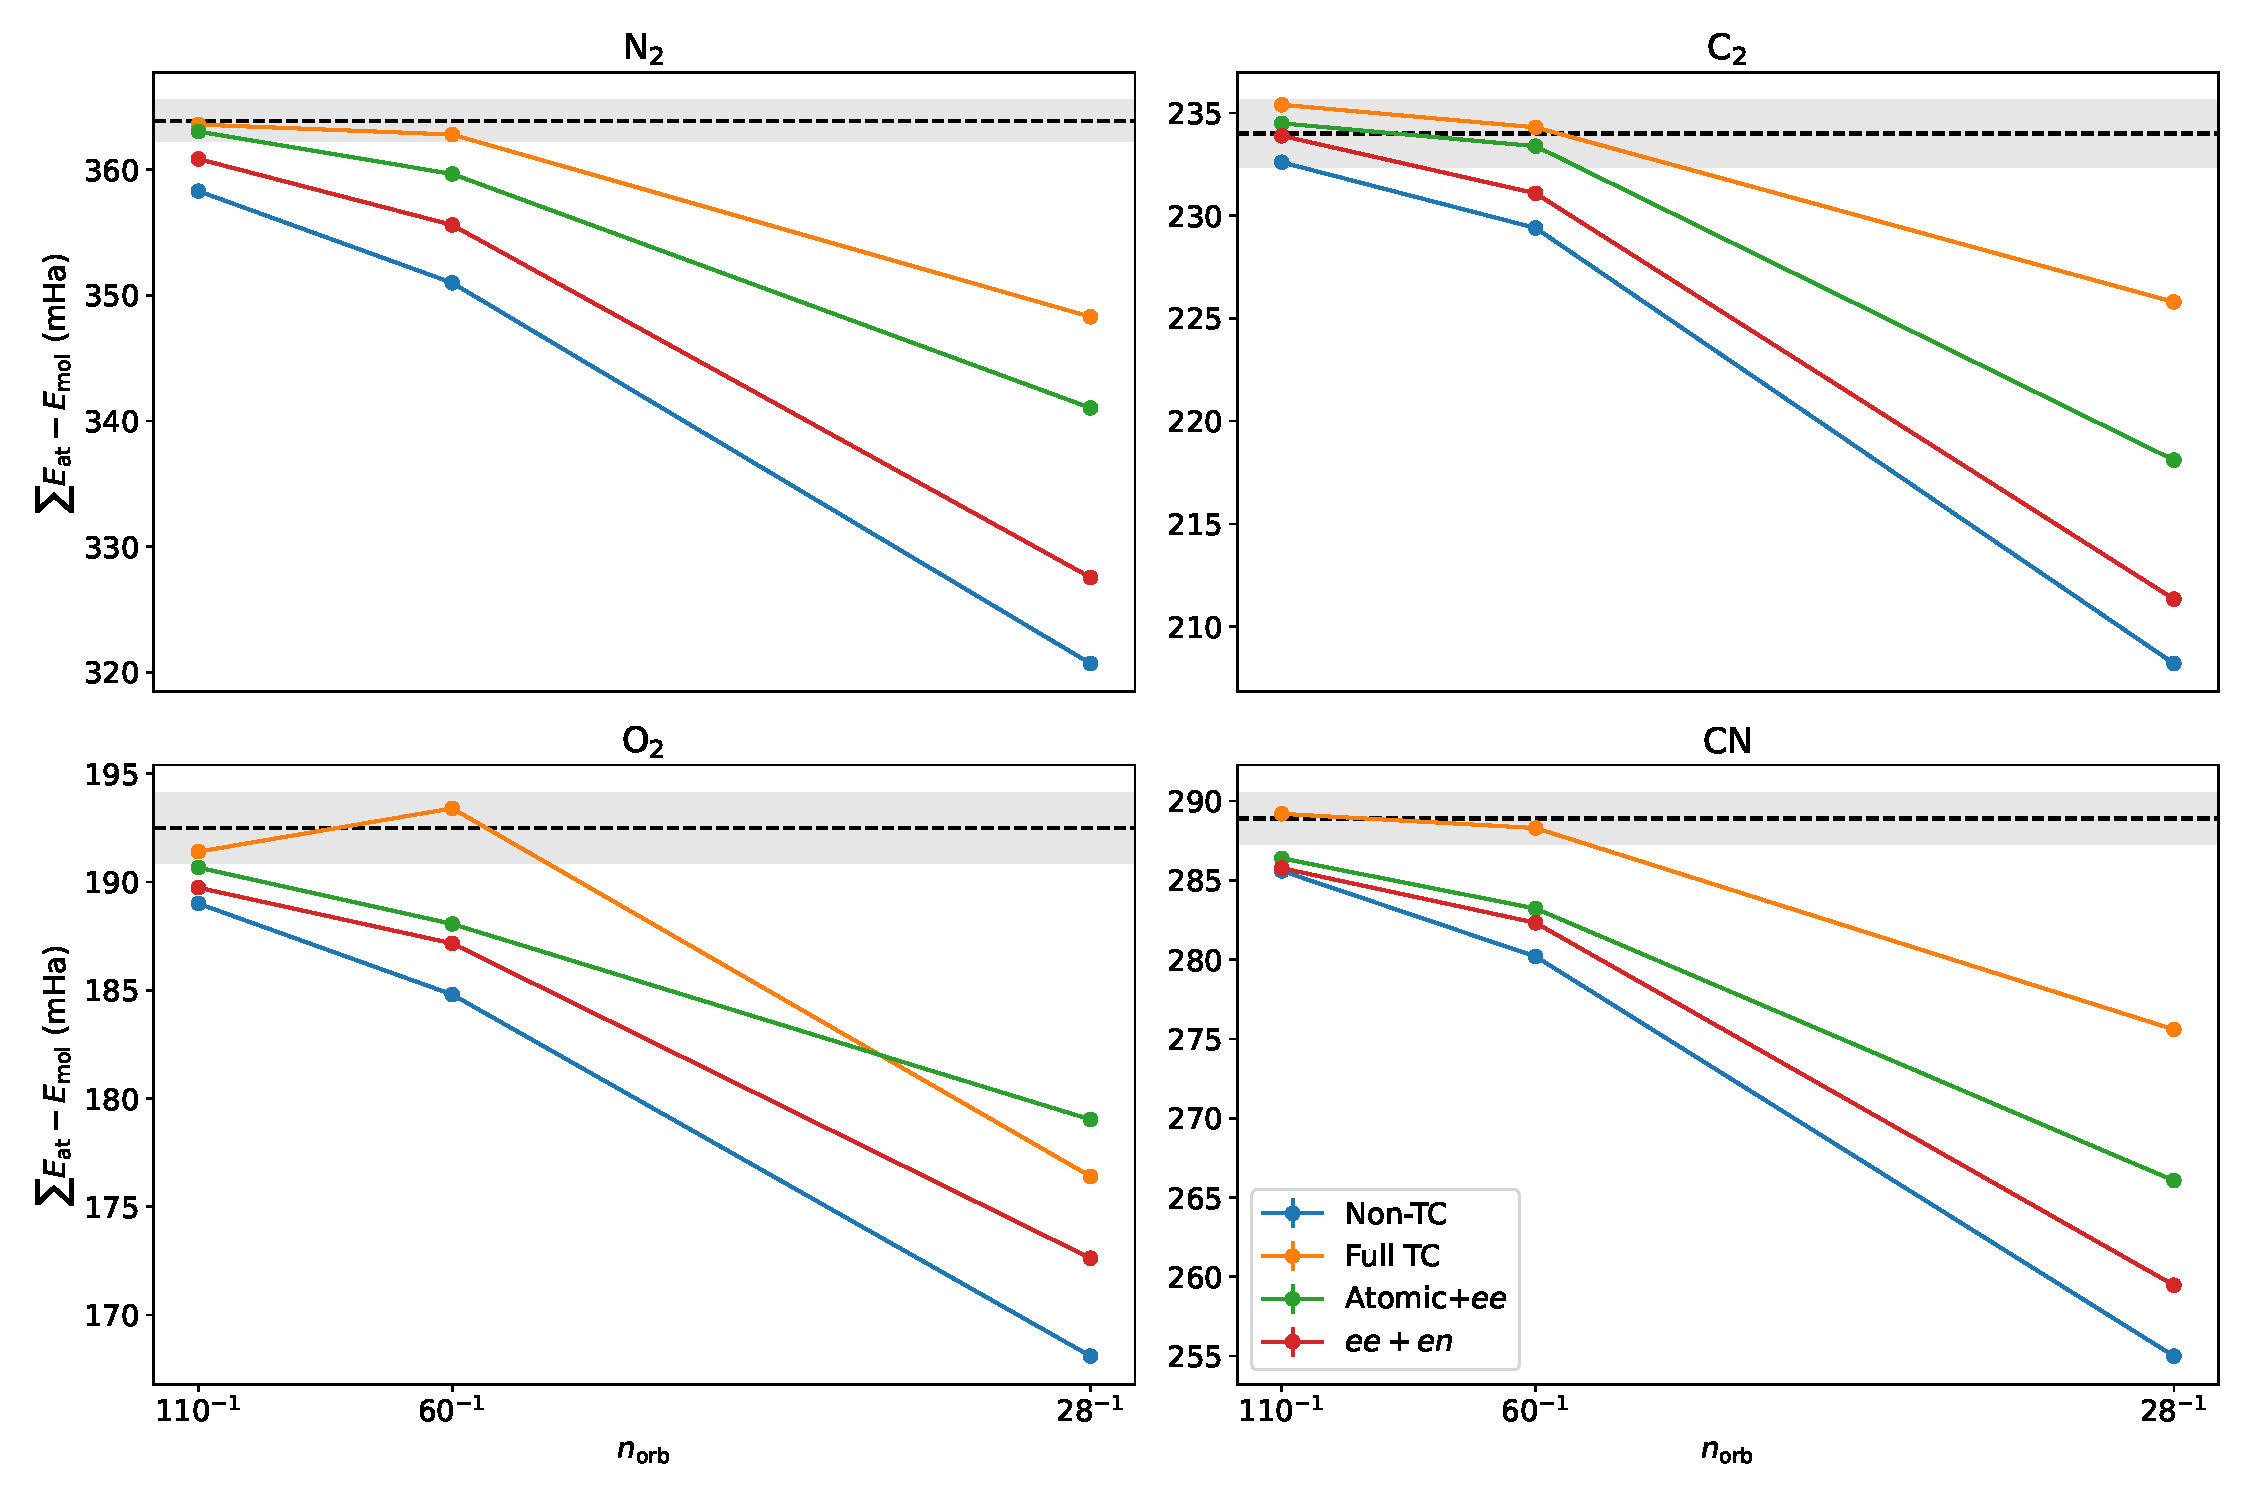
\includegraphics[width=\textwidth]{figures/universal/atomisation_energies}
    \caption{Atomisation energies for the molecules N$_2$, O$_2$, C$_2$ and CN as a function of the reciprocal of the number of orbitals. The CBS limit is represented by a dashed line and a grey region denotes the area within chemical accuracy ($\pm 1.6$ mHa) of this value. From these plots, we can see a consistent trend where the full TC treatment from \autoref{chap:opt} performs best in that it converges most rapidly to the CBS, with the atomic$+ee$ Jastrow factor approach also performing well. Interestingly, the $ee+en$ Jastrow factor approach also performs well, despite the undesirable absolute energies discussed in table \ref{tbl:universal-absE}, suggesting considerable error cancellation. In terms of atomisation energies, this approach also performs reasonably well, though the only data point within chemical accuracy is C$_2$ in the \vqz basis, but even non-TC is chemically accurate in this case.
    % \todo{should you move this to the discussion, out of the caption?}
    }
    \label{fig:universal-atomisation}
\end{figure}

\subsection{Binding Curves}

Here we report the N$_2$ binding curve with the \avtz basis set for the various choices of Jastrow factors. Values for the interatomic distance range between $1.92$ and $10$ Bohr. The Jastrow factors used were the atomic Jastrow factor, the atomic Jastrow factor with electron-electron terms optimised for the molecule (using a RHF or FCIQMC ansatz), and the minimal $ee$- and $ee+en$-Jastrow factors.  The binding curve for the FCIQMC-Jastrow factor (i.e. multideterminant ansatz with all terms optimised) from \autoref{chap:binding} is also shown for comparison. All choices of Jastrow factor give qualitatively correct binding curves.
Plots for the binding curves are shown in figure \ref{eq:binding-universal-zoom}, focusing on the minimum and dissociation regions. Compared to the FCIQMC-Jastrow factor of \autoref{chap:binding}, the binding curves using the Jastrow factors presented in this chapter shift the minimum upwards. This is to be expected, since we have fewer (or even no) parameters being optimised, and thus less flexibility in the VMC optimisation. Note that, while the cutoff $L$ for the minimal Jastrow factors is not optimised, its value was determined in section \ref{sec:universal-jastrow} based on this same system at equilibrium. Based on the results in section \ref{sec:universal-atomisation}, it is likely that this cutoff analysis effectively behaved as a surrogate for optimisation, and that $L=0.3$ Bohr would not be optimal for other systems, and may even result in values below the CBS limit. This suggests that simple Jastrow factors such as the $ee$-Jastrow factor are viable, but that they need to be used carefully, and may need to be optimised for each system.

\begin{figure}[htbp]
    \centering
    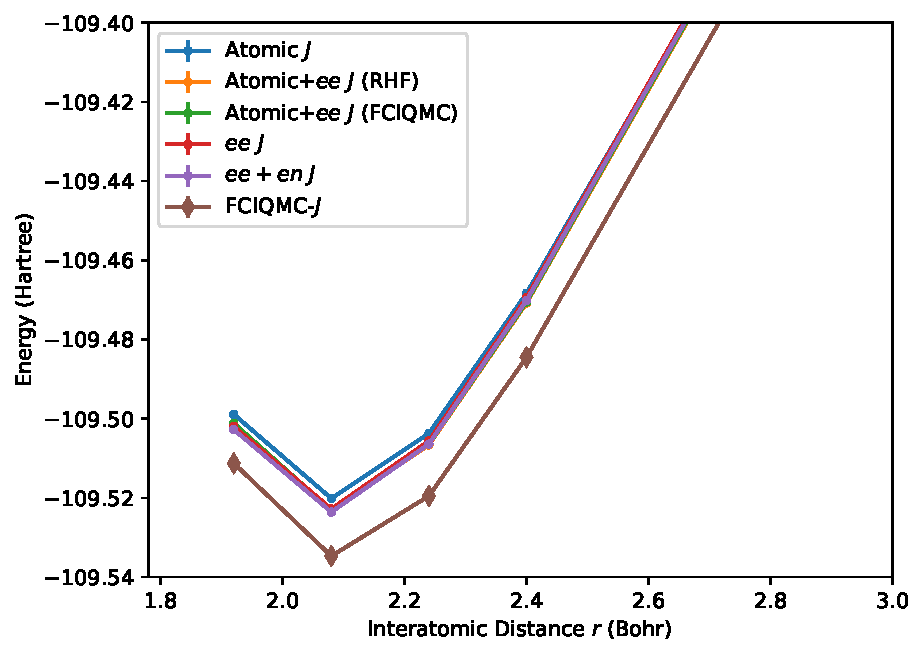
\includegraphics[width=0.9\textwidth]{figures/universal/n2_avtz_min}
    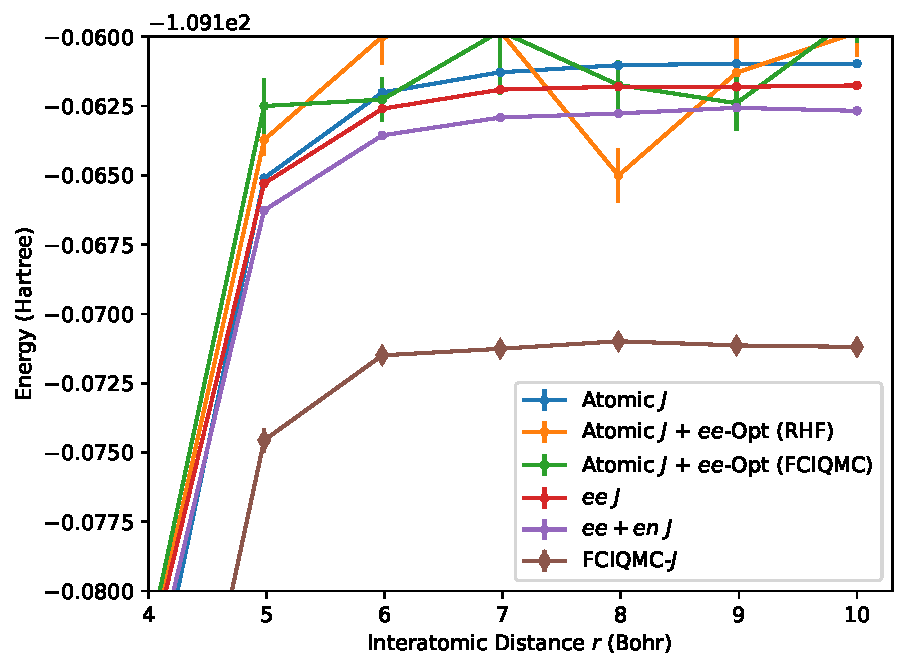
\includegraphics[width=0.9\textwidth]{figures/universal/n2_avtz_diss}
    \caption{Zoomed in plots of the N$_2$ binding curves for the various Jastrow factor choices. All forms give qualitatively correct binding curves. Included for comparison is the FCIQMC-Jastrow from \autoref{chap:binding}, which was shown to be good both at equilibrium and dissociation. Compared to this, all Jastrow factors newly presented in this chapter shift the minimum upwards, with all of them having similar values in this region except for the pure atomic Jastrow factor. This is likely because the eleectron-electron terms are suboptimal. Slight noise in the dissociated limit are likely connected to the error in the VMC optimisation, which was shown in \autoref{chap:opt} to be on the order of 0.1 mHa.
    % \todo{check the weird point at r=8.98 for the atomic+ee(RHF) Jastrow factor.}
    }
    \label{eq:binding-universal-zoom}
\end{figure}


It is also worth noting that unlike the RHF-Jastrow factor in \autoref{chap:binding}, the single-reference electron-electron optimisation with the atomic Jastrow factor performs well, and even gives the correct behaviour in the dissociated limit. This may be because the atomic Jastrow factor is already a good approximation for the dissociated limit, and so the electron-electron optimisation in the molecule does little extra work. It also does not have as much flexibility as the RHF-Jastrow factor from \autoref{chap:binding}, so the poor TC ansatz cannot do as much harm, though it is responsible for a higher energy estimate in the dissociated limit, as can be seen by comparing against the multireference (FCIQMC)-optimised electron-electron Jastrow factor.

\begin{figure}[htbp]
    \centering
    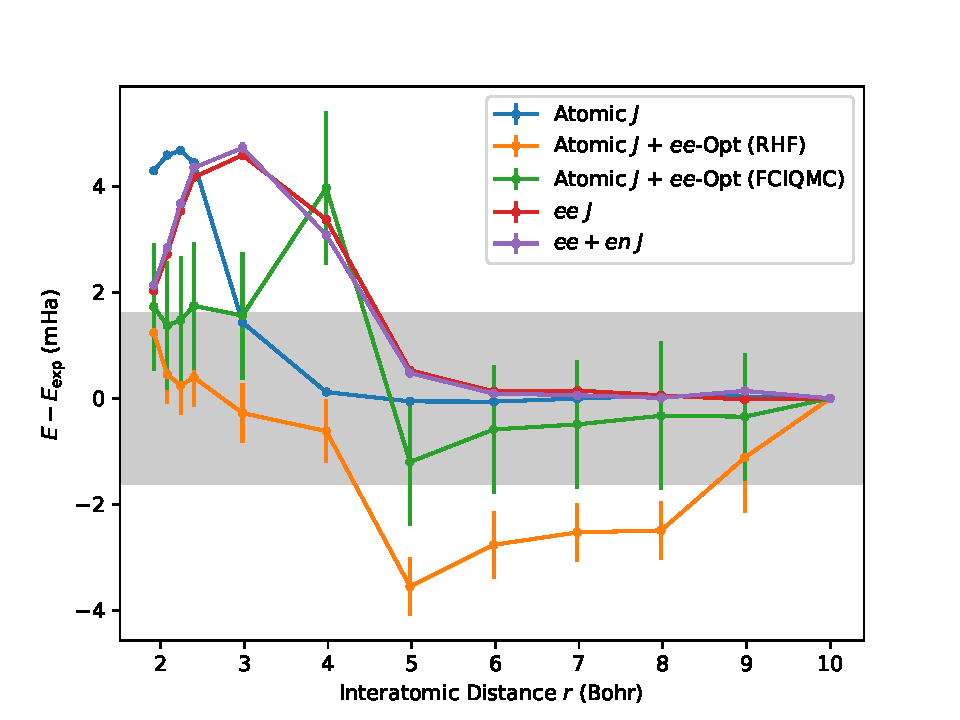
\includegraphics[width=\textwidth]{figures/universal/residuals}
    \caption{The binding curves relative to a fit to experimental data\supercite{leroyAccurate2006} for the nitrogen dimer, calculated in the \avtz basis for various Jastrow factor forms. All curves are normalised such that the value at $10$ Bohr is $0$ Hartree. The grey shaded area denotes a region of $\pm 1.6$ mHa (i.e. chemical accuracy). For reference, the multideterminantal FCIQMC-Jastrow from \autoref{chap:binding} is shown in brown (with diamonds). Both minimal Jastrow factor forms ($ee$ and $ee+en$, denoting with only electron-electron or with both electron-electron and electron-nucleus terms, respectively) stay above the experimental result, and are indeed very close to each other. The atomic Jastrow factors, whether containing $ee$ terms optimised for the molecule (RHF or FCIQMC as the $\Phi$ ansatz) or not optimised for the molecule (atomic $J$), have a less smooth behaviour, but are generally closer to the experimental result.
    % \todo{converge these and update the caption: the data for the two atomic+ee curves will change a little}
    }
    \label{fig:binding-universal-experiment}
\end{figure}

The energy estimates relative to experiment (normalised such that the energy at $10$ Bohr is $0$ Hartree) is shown in figure \ref{fig:binding-universal-experiment}. In contrast to the multireference Jastrow factors presented in \autoref{chap:binding}, such as the FCIQMC-Jastrow factor reproduced here, the atomic and minimal Jastrow factors stay above the experimental result and converge relatively monotonically. That said, they are overall not as close to the experimental result as the FCIQMC-Jastrow factor across the binding curve. It is also worth noting that the $ee$- and $ee+en$-Jastrow factors result in very similar curves, suggesting only a minimal effect from the nuclear term.

Since all of these Jastrow factors are strongly localised, we expect them all to be well-behaved at long interatomic separation, i.e. they should be size consistent, and that is consistent with figure \ref{fig:binding-curves-experiment}. The possible exception is the single-determinant-optimised atomic$+ee$ Jastrow factor, as the electron-electron term is optimised with a non-size-consistent wave function ansatz. Howeer, as observed even this curve appears well-behaved. We approximate the size consistency error by the difference in energies between the molecule and the sum of its parts and show the results in table \ref{tbl:size-consistency-uni}. Indeed, we find all Jastrow factors to be size consistent, comparable to MRCI-D-F12.

\begin{table}[htbp]
    \centering
    \begin{tabular}{c|c}
        Jastrow Factor & $\sum E_\mathrm{atom} - E_\mathrm{molecule}(r=10)$ (mHa) \\
        \hline
        Atomic & -0.2(0) \\
        Atomic+$ee$ (RHF) & 0.5(0) \\
        Atomic+$ee$ (FCIQMC) & 0.9(0)\\
        $ee$ & -0.6(0) \\
        $ee+en$ & -0.6(1) \\
        \bottomrule
        % Non-TC & -3.9(1) \\
        MRCI-D-F12 & -0.9
    \end{tabular}
    \caption{
        Size consistency error, measured as the difference between the sum of energies for the constituent atoms in isolation and the energy of the molecule at dissocation (taken to be $10$ Bohr). We see that all methods presented here have size consistency errors that are comparable to MRCI-D-F12.
    }
    \label{tbl:size-consistency-uni}
\end{table}

Finally, the atomisation energy estimates using the binding curves, i.e. the difference between the energy in the dissociated limit and that at equilibrium, are shown in table \ref{tbl:binding-atomisation-energies-uni}. All Jastrow factors perform similarly well, comparable to MRCI-D-F12. While not as accurate as previous methods presented in this dissertation, these approaches have fewer parameters to optimise.

\begin{table}[htbp]
    \centering
        \begin{tabular}{c|c}
            Jastrow Factor & Atomisation Energy (mHa) \\
            \hline
            Atomic & 358.9(0) \\
            Atomic+$ee$ (RHF) & 361.8(0) \\
            Atomic+$ee$ (FCIQMC) & 361.7(0)\\
            $ee$ & 361.0(0) \\
            $ee+en$ & 360.3(1) \\
            \bottomrule
            MRCI-D-F12 & 359.5 \\
            HEAT\supercite{fellerSurvey2008} & 363.9 \\
            Experiment\supercite{leroyAccurate2006} & 363.7
        \end{tabular}
    \caption{Atomisation energies for the nitrogen dimer using only the binding curve. We see that all methods presented here have atomisation energies that are comparable to MRCI-D-F12, with most slightly outperforming it. While not within chemical accuracy like full TC or the multireference Jastrows presented in \autoref{chap:binding}, these results are still promising on account of their relative simplicity.
    }
    \label{tbl:binding-atomisation-energies-uni}
\end{table}

\section{Conclusion and Outlook}

We have presented an alternative approach to constructing Jastrow factors, either using a minimal approach focusing on describing analytical behaviour near coalescence points, or reusing Jastrow factors optimised for small systems (such as an atom) for larger systems (such as a molecule). We have shown that the resulting Jastrow factors are size consistent and provide rapid basis set convergence when compared against conventional electronic structure methods.
These updated workflows represent significant improvements in the scalability and ease of use for TC methods, while arguably being more conceptually satisfying by making the Jastrow factors more general.

It is, however, worth pointing out some shortcomings of these approaches. Perhaps the most obvious shortcoming is the relative lack of flexibility in the Jastrow factor, as either there are no terms to optimise or relatively few compared to previous approaches presented in this dissertation. Moreoever, with the exception of the atomic$+ee$ Jastrow factor with the electron-electron term optimised using an FCIQMC ansatz, there is no clear way for these methods to be tailored for specific states. Additionally, the use of minimal Jastrow factors may lead to TC energies well below the CBS limit if not careful in the choice of the cutoff function. While these appear to be mostly compensated for by error cancellation when computing atomisation energies, the nonmonotonic convergence to the CBS limit is nevertheless undesirable. This suggests future studies on the effects of the cutoffs and the potential need for optimising its parameters for each state. In this sense, the form of the minimal Jastrow factor may be ``universal'', but its cutoffs may not be. Since this convergence appears strongly linked to the core region, it may also be worthwhile studying the effects of using futher core functions, or \glspl{ECP}, as well as a more careful introduction of the electron-electron-nucleus term in the Fournais-Jastrow factor.

These results suggest that a realistic approach to studying larger systems, or performing optimisation deterministically, with the transcorrelated method would involve combining Jastrow factors optimised for small systems and reoptimising some terms (such as the electron-electron term) for the larger system, as a form of correction. This would allow for a more computationally tractable approach with fewer optimisable parameters, while still benefiting from rapid convergence to the CBS limit.
